\documentclass[9pt,twocolumn,twoside]{pnas-new}
% Use the lineno option to display guide line numbers if required.

\articletype{NEUROSCIENCE}%%%% Article topic/classification

\templatetype{pnasresearcharticle} % Choose template
% {pnasresearcharticle} = Template for a two-column research article
%\templatetype{pnasmathematics} %= Template for a one-column mathematics article
% {pnasinvited} %= Template for a PNAS invited submission


\begin{document}


\title{Model-based inference of reward identity in the lateral orbitofrontal cortex}

% Use letters for affiliations, numbers to show equal authorship (if applicable) and to indicate the corresponding author


\author[a]{Qingfang Liu}
\author[b]{Yao Zhao}
\author[c]{Taaseen Khan}
\author[a]{Nicole Moussa}
\author[a]{Geoffrey Schoenbaum}
\author[a,1]{Thorsten Kahnt}

\affil[a]{National Institute on Drug Abuse Intramural Research Program, Baltimore, MD 21224, USA}
\affil[b]{Department of Psychology, University of Pennsylvania,
Philadelphia, PA 19104, USA}
\affil[c]{Feinberg School of Medicine, Northwestern University,
Chicago, IL 60611, USA}

% Please give the surname of the lead author for the running footer
\leadauthor{Kahnt}

% Please add a significance statement to explain the relevance of your work
\significancestatement{Adaptive decisions often require inferring the consequences of choices that have never been directly experienced. Here, we show that such inference can recover the identity of a specific expected reward, not merely whether an outcome is good or bad. We further find that the lateral orbitofrontal cortex preferentially represents reward identity when it must be inferred through learned associations rather than recalled from direct experience. These findings suggest that the brain does not represent all outcome information equally but instead prioritizes detailed information when it is most useful for guiding behavior.}

% Please include corresponding author, author contribution and author declaration information
\authorcontributions{Q.L., Y.Z., G.S., and T. Kahnt designed research; Q.L., Y.Z., T. Khan, and N.M. performed research; Q.L. and T. Kahnt analyzed data; Q.L. developed the theoretical model; G.S. and T. Kahnt supervised research; Q.L. wrote the original draft; and all authors reviewed and edited the manuscript.}

\authordeclaration{The authors declare no competing interest.}
\correspondingauthor{\textsuperscript{1}To whom correspondence should be addressed. E-mail: thorsten.kahnt@nih.gov}

% At least three keywords are required at submission. Please provide three to five keywords, separated by the pipe symbol.
\keywords{goal-directed behavior $|$ cognitive map $|$ orbitofrontal cortex $|$ outcome-guided behavior $|$ resource-limited model}

\begin{abstract}
Flexible behavior requires using learned relationships to infer outcomes that have not been directly experienced. It remains unclear whether such inference retrieves only scalar value or the identity of a specific expected outcome. We combined sensory preconditioning, selective outcome devaluation, and functional MRI to test the content and neural representation of inferred outcomes in humans. Participants first learned associations between pairs of visual cues and then learned that the second cue of each pair predicted a specific food odor. After selective satiation reduced the value of one of the food odors, choices decreased not only for cues directly associated with that odor but also for preconditioned cues whose outcomes had to be inferred through the associative structure. This transfer of devaluation indicates that model-based inference recovers the specific identity of outcomes rather than their cached value. Importantly, multivariate analyses of fMRI responses to preconditioned cues revealed inferred outcome-identity representations in the lateral orbitofrontal cortex (OFC). Outcome-identity representations in this region were not significant for conditioned cues. To account for this pattern, we propose a resource-limited framework in which explicit outcome identities receive greater representational resources when they provide greater computational benefit. Together, these findings show that human model-based inference accesses specific reward identities and suggest that lateral OFC may prioritize outcome information according to its computational utility.
\end{abstract}

\dates{This manuscript was compiled on \today}
\doi{\url{www.pnas.org/cgi/doi/10.1073/pnas.XXXXXXXXXX}}


\maketitle
\thispagestyle{firststyle}
\ifthenelse{\boolean{shortarticle}}{\ifthenelse{\boolean{singlecolumn}}{\abscontentformatted}{\abscontent}}{}

\Firstpage

%The \Firstpage command is used to format the first page text column size. The same size will be maintained for subsequent paragraph until the \Endparasplit or \Parasplit command is encountered.



Model-based behavior requires mental simulation of outcomes that have never been
directly experienced \cite{daw2011model,doll2015model,wangkahnt21}. Rather than relying only on cached values learned through direct reinforcement, animals can infer the likely consequences of a choice by combining separately learned associations. Such model-based inference supports adaptive behavior when outcomes change, while impairments in this process may contribute to maladaptive or compulsive behavior, including substance use disorders \cite{kahsch21,kahnt2023computationally}. Sensory preconditioning (SPC) provides a behavioral framework for studying such inference \cite{kahnt2023computationally,jones12,wang2020interactions}. In a typical SPC procedure, neutral cue pairs are first learned (A $\rightarrow$ B, C $\rightarrow$ D), after which the second cue from each pair is directly conditioned with an outcome (B $\rightarrow$ reward, D $\rightarrow$ no reward). During a subsequent probe test without feedback, responding to A over C indicates that subjects have inferred the outcome associated with B from the learned A--B and B--reward associations.

Prior work indicates that the orbitofrontal cortex (OFC) is necessary for responding to preconditioned but not directly conditioned cues during the probe phase. For example, inactivating the OFC in rats during the probe test leaves responding to B, which was directly associated with reward, intact, while selectively impairing responding to A, which requires inferring the associated reward \cite{jones12}. Consistent findings have been observed in humans: combining the SPC task with transcranial magnetic stimulation (TMS) targeting the OFC network selectively disrupted inference-based responding during the probe test without affecting direct reward learning \cite{wang2020targeted}. Together, these results provide cross-species evidence for a role of the OFC in model-based inference.

\Parasplit

However, it remains unclear what information is inferred during SPC. In particular, behavioral responses to preconditioned cues could reflect inference of a scalar outcome value or retrieval of a more specific outcome identity. The former possibility is that SPC supports inference over reward value: a cue may come to predict that ``something good'' or ``something bad'' will occur. The latter possibility is that subjects infer a specific reward: a cue may predict a specific outcome, such as a particular food odor, whose value can later be updated. Given extensive evidence that lateral OFC represents the identity of expected rewards \cite{howard2015identity,howard2017identity,howard2018identity,howard2021specific,liuyaoatt24,witkowski2026identity}, this possibility raises a further question: does lateral OFC represent inferred and directly learned outcome identities in the same manner?


Selective outcome devaluation provides a direct test of the question whether cached value or outcome identity is expected \cite{HowRey2020,liu2025distinct,hart20}. In this procedure, after learning an association between a cue and a specific reward, the value of that reward is reduced through selective satiation or conditioned taste aversion. If responding to the cue depends on the expectation of a specific outcome, devaluing that outcome should reduce responding to cues that predict it. In contrast, if responding is driven by a cached scalar value that is not linked to the specific outcome identity, devaluing the outcome should have little or no effect on responding to the cue.




In the current work, we combined sensory preconditioning \cite{Brogden39} with outcome devaluation \cite{HowRey2020,liu2025distinct} to assess if inferred cue-outcome pairings are sensitive to devaluation. Participants learned associations between pairs of visual cues as well as between the second cues and one of two food odors before completing two probe tests, with a selective satiation procedure between the two probe tests to reduce the pleasantness of one of the food odors. Behaviorally, we asked whether devaluation changes choices for both directly conditioned and preconditioned cues, and whether these changes track individual changes in odor pleasantness. Neurally, we tested whether cue-evoked activity patterns in the OFC reflect outcome value or identity. We found, first, that devaluation altered choices for both directly conditioned and preconditioned cues, indicating that inference involves specific outcome identity rather than only cached value. Second, pattern-based fMRI analyses revealed that lateral OFC preferentially represented reward identity for preconditioned compared to conditioned cues, suggesting that outcome-identity representations are prioritized according to their computational utility. We propose a resource-limited framework model to account for the preferential representation of inferred outcomes in lateral OFC.





\begin{figure*}[t]
\centering
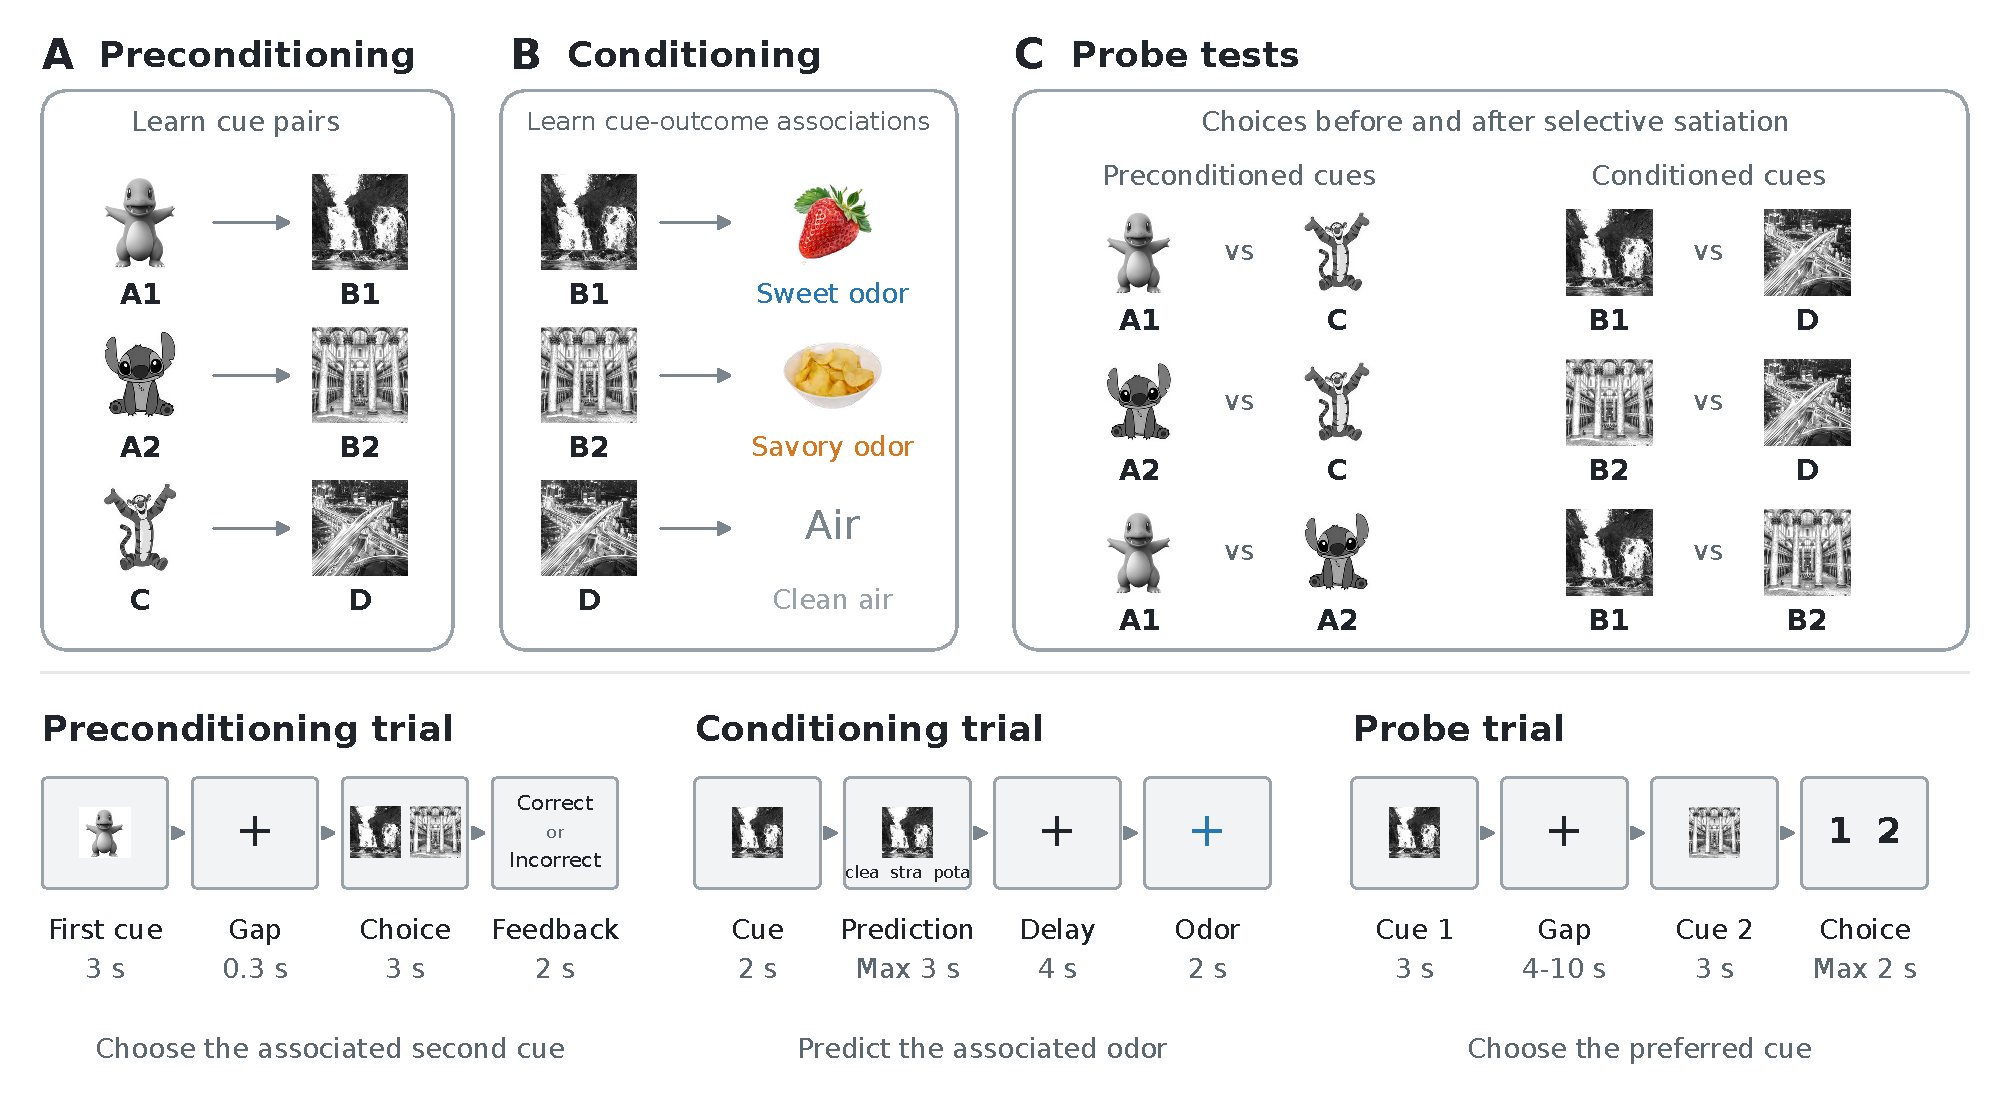
\includegraphics[width=0.95\linewidth]{../../fig/fig_design_python.pdf}
\caption{\textbf{Experimental design.} 
\textbf{A. Preconditioning.} Participants learned associations between pairs of visual cues, where the first cue served as the preconditioned cue (A1, A2, C) and the second as the conditioned cue (B1, B2, D). On each trial, the first cue was shown for 3\,s, followed by a 0.3\,s gap and then a 3\,s choice display with two possible second cues—the correct associate and one alternative from the same cue set. Participants indicated the associated cue via left/right keypress. Feedback (correct or incorrect) was displayed for 2\,s within the jittered 3--8\,s inter-trial interval, followed by fixation for the remainder of that interval. The mapping of stimulus type (character vs.\ place) to first/second cue positions was counterbalanced across participants.
\textbf{B. Conditioning.} Participants learned associations between the conditioned cues and their outcomes: two equally preferred food odors (one sweet, one savory) and clean air. The food odor predicted by B2 was later selectively devalued by having participants consume a meal matching that odor. Each trial began with a 2\,s presentation of a conditioned cue, followed by a 3\,s prediction period in which the cue remained on the screen alongside three abbreviated odor names. Participants indicated their predicted outcome. After a 4\,s delay, the associated odor (or clean air) was delivered for 2\,s. Trials ended with a jittered 4--10\,s inter-trial interval.
\textbf{C. Probe test.} Before and after the meal, participants made choices between pairs of cues to assess preferences. Each trial began with a 3\,s presentation of the first cue (cue\,1), followed by a jittered 4--10\,s interval before the second cue (cue\,2) appeared for 3\,s. Participants then had 2\,s to indicate their choice, after which the trial ended with a jittered 4--10\,s inter-trial interval.
}
\label{fig-design}
\end{figure*}




\section*{Results}
\label{sec-res}


\subsection*{Experimental design}
\label{subsec-design}



During preconditioning (\autoref{fig-design}A), participants learned associations between pairs of visual cues, where the first cue in a pair is referred to as the preconditioned cue (A1, A2, C), and the second cue is the conditioned cue (B1, B2, D). Next, during conditioning (\autoref{fig-design}B), participants learned associations between conditioned cues and two specific food odor rewards (one savory, one sweet, equally preferred) as well as clean air. This was followed by two probe tests (\autoref{fig-design}C), in which preferences for all cues were assessed. The two probe test sessions were separated by a devaluation procedure, in which participants consumed a meal matching the food odor predicted by B2. The meal-matched and non-matched odors are referred to as the devalued and non-devalued odors, respectively.

Previous work has shown that consuming a meal matching a food odor selectively devalues this food odor but leaves the value of non-matched food odors intact \cite{howard2017identity,HowRey2020,liu2025distinct}. This leads to a change in preference from the pre- to the post-devaluation probe test, such that after the meal, participants prefer conditioned cues associated with the non-devalued food odor over cues associated with the devalued food odor \cite{HowRey2020,liu2025distinct}. However, it is unknown whether this devaluation also transfers to the preconditioned cues. Answering this question gives insights into the content of the inference. If preferences for preconditioned cues changed in the same way as for conditioned cues, this would indicate that inference acts on specific outcomes. In contrast, if there is no change in preferences, this would indicate that participants infer the cached reward value that they previously learned for conditioned cues.




\subsection*{Outcome devaluation reduces choices for conditioned and preconditioned cues}
\label{subsec-beh}


Participants showed a clear learning pattern across runs during preconditioning (\autoref{fig-beh}A), with accuracy increasing from the initial training ($0.81 \pm 0.11$) to the final run ($0.99 \pm 0.03$; mean $\pm$ SD). Accuracy did not differ across the three cue pairs (A1--B1, A2--B2, and C--D; Friedman test: $\chi^2(2) = 0.29$, $p = 0.867$). During conditioning (\autoref{fig-beh}B), accuracy of odor predictions also improved steadily across runs. By the final run, all participants reached at least 0.75 accuracy (mean $\pm$ SD $= 0.94 \pm 0.069$), and final accuracy did not differ among cues B1, B2, and D (Friedman test: $\chi^2(2) = 3.887$, $p = 0.143$).


We confirmed the effectiveness of our selective satiation procedure by analyzing changes in odor pleasantness ratings from before to after the meal (\autoref{fig-beh}C). The devalued odor showed a significant decrease in pleasantness following the meal ($W = 30.0$, $p < 0.001$; Wilcoxon signed-rank test), whereas pleasantness ratings for the non-devalued odor did not change significantly ($W = 127.5$, $p = 0.139$). The pre-to-post decrease was significantly greater for the devalued than the non-devalued odor ($t(29) = -3.42$, $p < 0.001$; one-sided paired $t$-test), consistent with a sensory-specific satiety effect. There was also no significant change in pleasantness ratings for clean air ($W = 54.0$, $p = 0.286$).


Importantly, in line with previous work \cite{HowRey2020,liu2025distinct}, this selective devaluation affected choices during the probe test. Choice proportions for conditioned cues associated with the devalued food odor (B2) decreased after the meal, both in the $B2>B1$ ($p = 0.0021$) and $B2>D$ choice pairs ($p = 0.0168$; \autoref{fig-beh}D). Choices for the conditioned cue associated with the non-devalued food odor showed no significant change from pre- to post-meal ($B1>D$: $p = 0.5309$). The pre-to-post decrease was significantly greater for $B2>D$ than for $B1>D$ ($t(30) = -1.72$, $p = 0.048$; one-sided paired $t$-test).

Critically, we observed a similar pattern for preconditioned cues indirectly associated with the devalued food odor (A2), such that participants were less likely to select A2 in both the $A2>A1$ ($p = 0.0021$) and $A2>C$ choice pairs ($p = 0.0069$; \autoref{fig-beh}E), with no significant change from pre- to post-meal for $A1>C$ ($p = 0.1972$). The pre-to-post decrease was numerically greater for $A2>C$ than for $A1>C$, but this difference was not significant ($t(30) = -1.23$, $p = 0.115$; one-sided paired $t$-test). These results are consistent with devaluation transfer to preconditioned cues and access to specific outcome information, although evidence for the selectivity of this transfer remains limited.



\begin{figure*}[t]
\centering
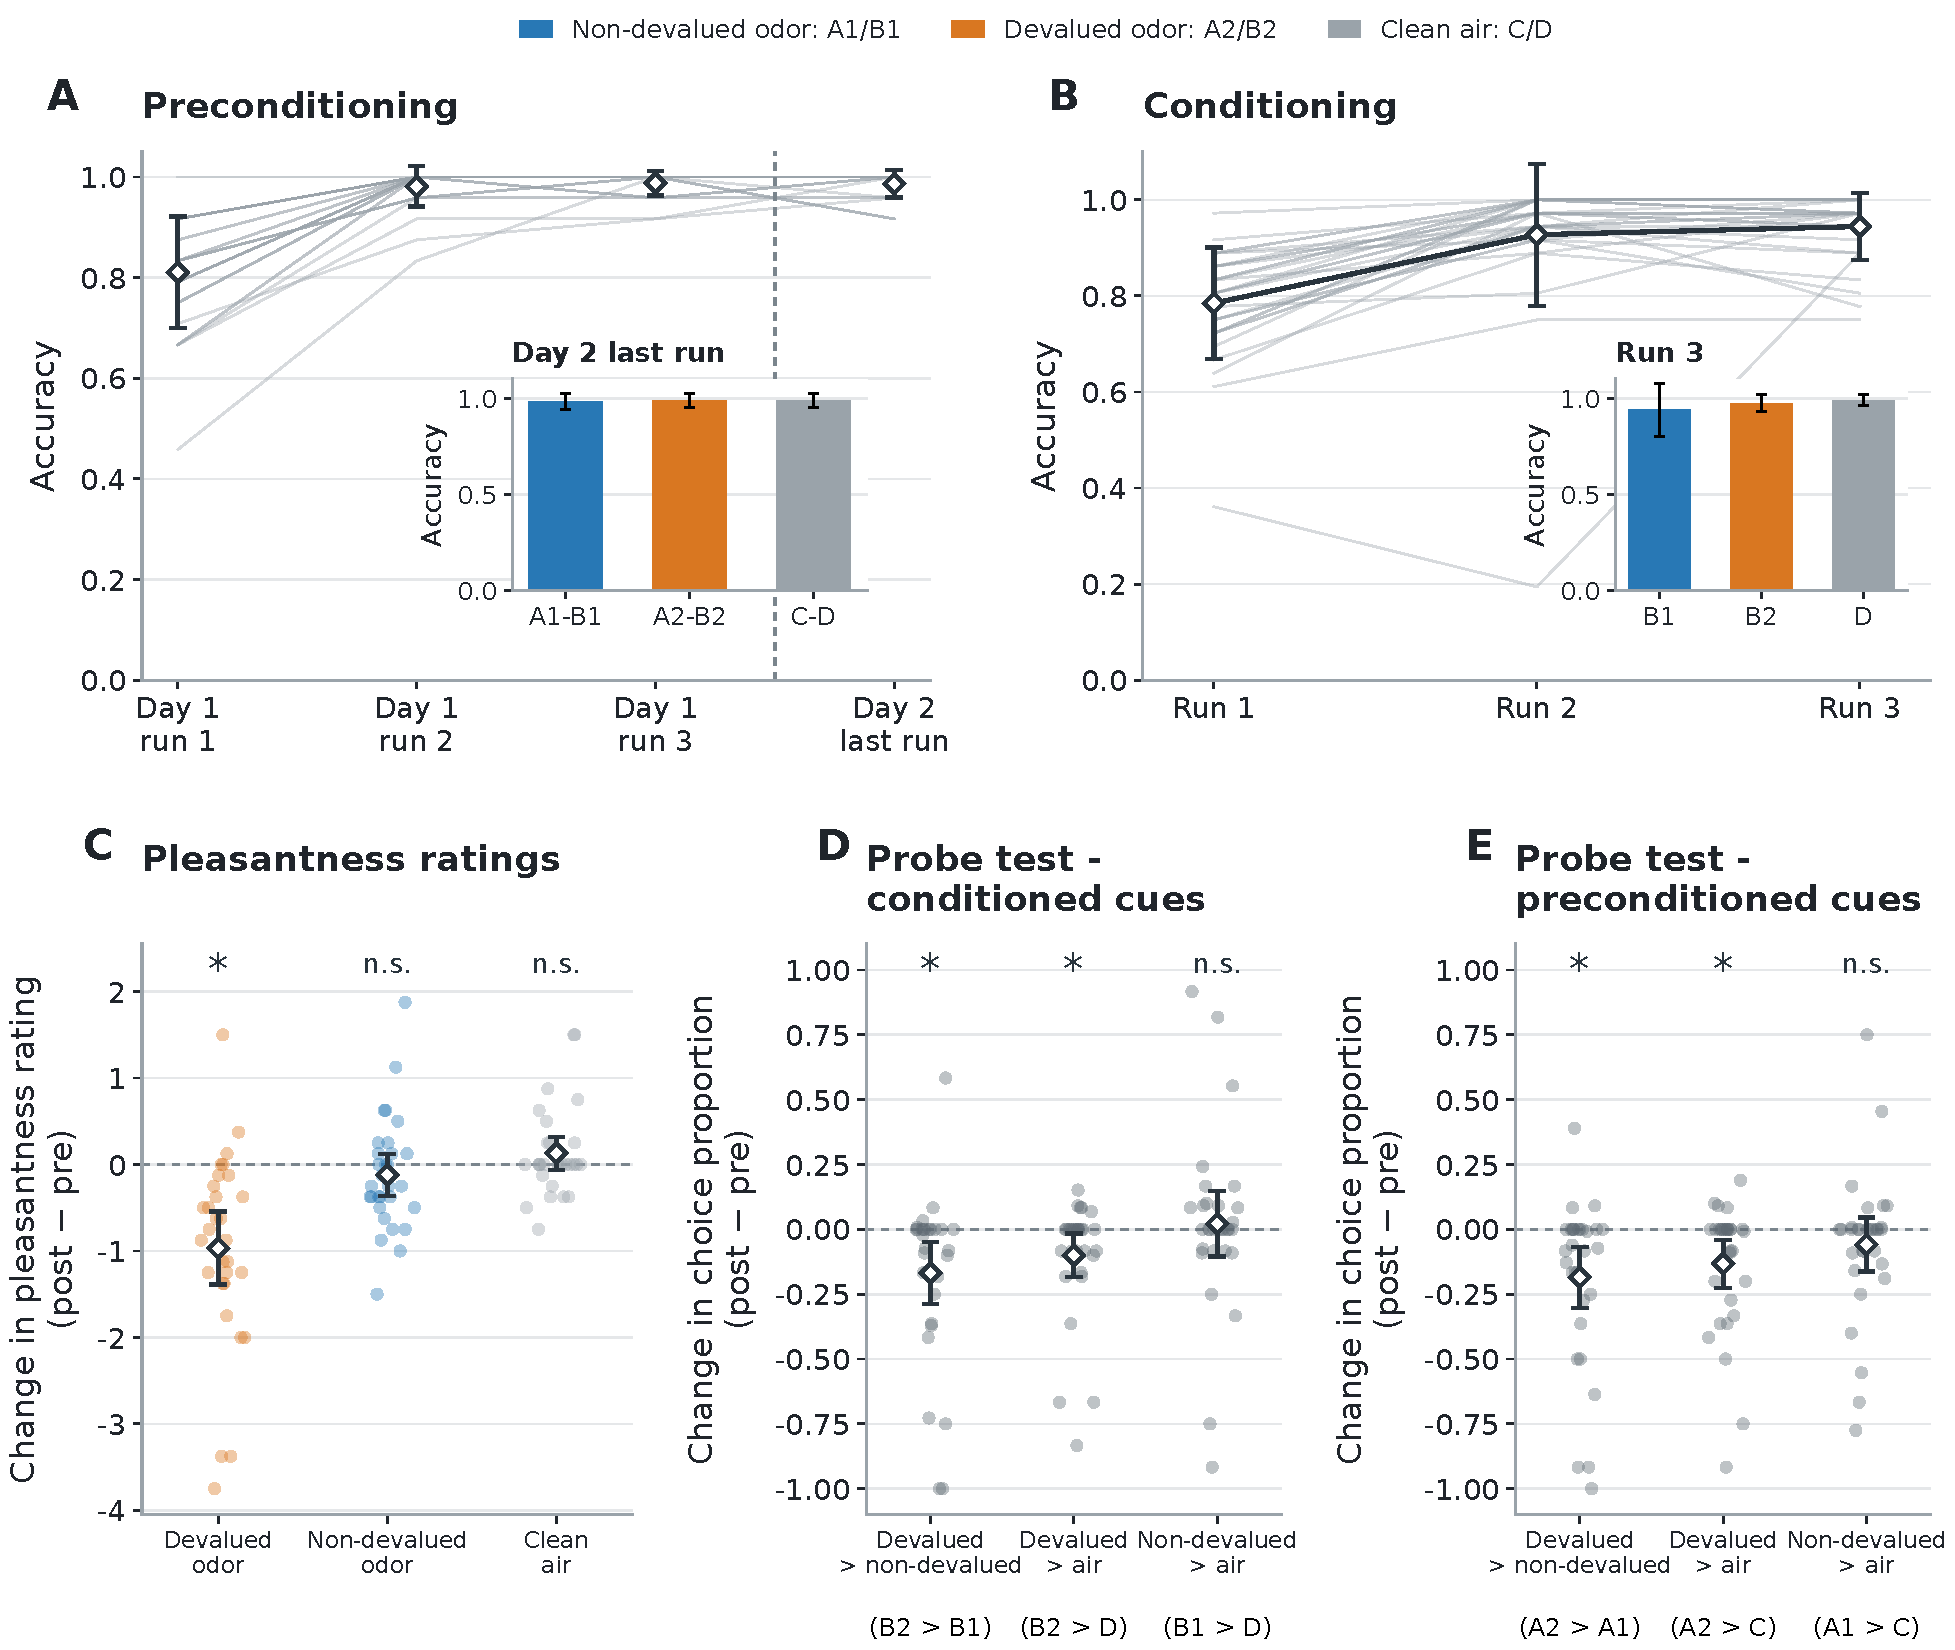
\includegraphics[width=0.95\linewidth]{../../fig/fig_behavior.pdf}
\caption{
\textbf{Direct and transferred outcome devaluation.}
\textbf{A. Preconditioning accuracy across runs.} Open diamonds indicate mean accuracy with standard-deviation bars; thin gray lines show individual participants. Inset shows mean accuracy with standard-deviation bars for the three pair types (A1--B1, A2--B2, C--D) in the final preconditioning run. Color denotes cue pairs later associated with non-devalued odor (blue), devalued odor (orange), and clean air (gray).
\textbf{B. Conditioning accuracy across runs.} Dots represent individual participants; connected open diamonds indicate mean accuracy with standard-deviation bars across the three runs. Inset shows mean accuracy with standard-deviation bars for B1, B2, and D in the final conditioning run. Color code as in A.
\textbf{C. Odor pleasantness changes from pre- to post-devaluation.} Negative values indicate reduced pleasantness after the meal. Pleasantness ratings decrease more for meal-matched than non-matched odors.
\textbf{D. Probe test - conditioned cues.} Choice proportion is defined as selecting the cue listed first over the cue listed second in a pair (e.g., $B2>B1$). The y-axis shows the post-meal minus pre-meal change in this proportion with negative values indicating reduced preference for the first cue named in each comparison. Dots represent individual participants, open diamonds indicate means, and error bars show t-based 95\% confidence intervals.
\textbf{E. Probe test - preconditioned cues.} Data as in D but for preconditioned cues. All analyses include 31 participants, except for pleasantness ratings (30 participants because one participant's ratings were unavailable). Asterisks denote uncorrected $p < 0.05$ from two-sided Wilcoxon signed-rank tests of paired changes against zero; n.s., not significant.
}
\label{fig-beh}
\end{figure*}



\subsection*{Lateral OFC represents inferred reward identity}


Our behavioral findings indicate that participants inferred specific outcome identities from preconditioned cues. We next asked where these inferred outcome identities are represented in the brain. Given previous evidence that OFC activity evoked by conditioned cues represents the identity of expected rewards \cite{howard2015identity,howard2017identity}, we tested whether preconditioned cues also evoke representations of their inferred food odors in OFC. We used representational similarity analysis (RSA) to test whether cues predicting the same odor elicited more similar neural activity patterns than cues predicting different odors (\autoref{fig-fmri}B). Analyses used two independently defined bilateral OFC regions, labeled lateral and medial OFC (\autoref{fig-fmri}A) \cite{kahnt2012connectivity}. We analyzed responses to the first cue presented on each trial during the premeal probe test, separately for conditioned and preconditioned cues, excluding cues associated with clean air. Neural pattern comparisons were restricted to cue presentations from different runs. In lateral OFC, neural patterns evoked by preconditioned cues reflected the identities of their associated food odors (mean Spearman $\rho = 0.029$, $t(30) = 2.35$, $p = 0.013$; \autoref{fig-fmri}C).

The RSA results suggest that lateral OFC represents the identities of inferred odors. We next asked whether these representations are shared with those evoked by smelling the odors themselves. To test this, we used cross-task decoding, training a classifier to distinguish odor identities from neural responses during odor smelling and testing it on cue-evoked responses during the premeal probe test (\autoref{fig-fmri}D). The classifier successfully decoded the expected odor identities from responses to preconditioned cues in lateral OFC (decoding accuracy = 54.10\%; chance = 50\%; $t(30) = 2.22$, $p = 0.017$; \autoref{fig-fmri}E). For conditioned cues, neither analysis detected significant odor-identity information in either OFC region (all $p > 0.05$; \autoref{fig-fmri}C,E). Odor-identity effects for preconditioned cues also did not reach significance in medial OFC (RSA: $p = 0.186$; decoding: $p = 0.084$). The cross-task decoding result in lateral OFC supports the interpretation that preconditioned cues reinstated neural representations shared with the direct sensory experience of their associated odors.



\begin{figure*}[t]
\centering
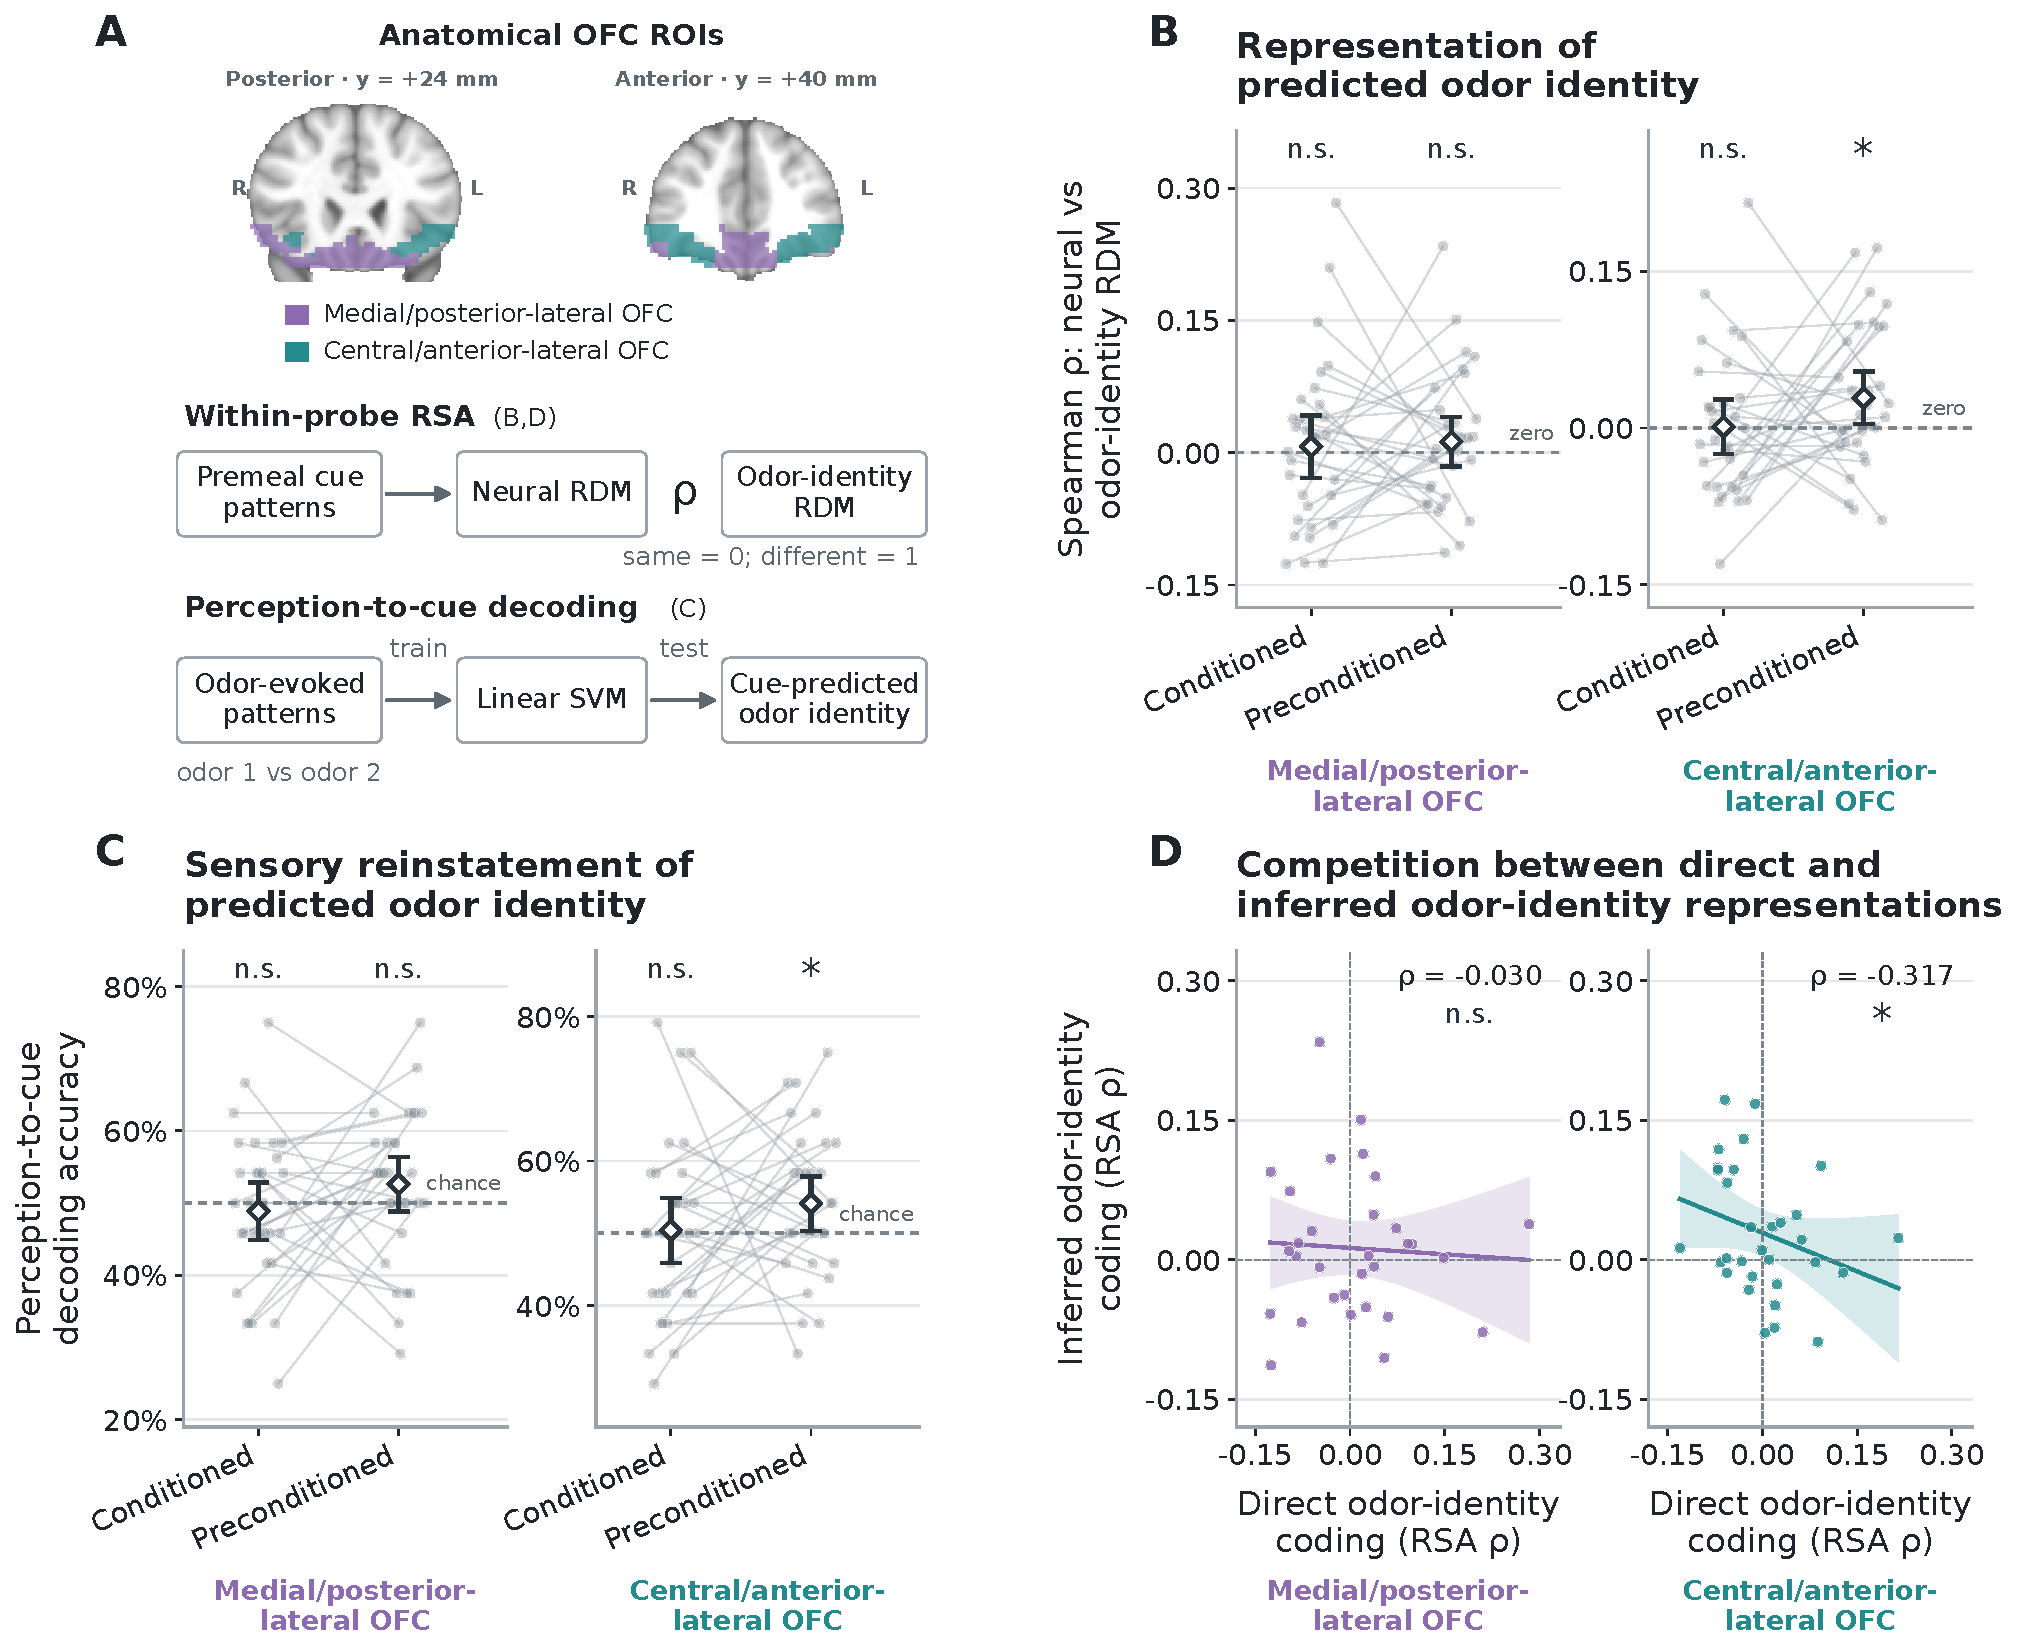
\includegraphics[width=0.95\linewidth]{../../fig/odor_identity_fmri.pdf}
\caption{
\textbf{Lateral OFC represents inferred reward identity.}
\textbf{A. Independently defined OFC regions.} Coronal views at MNI $y = 24$ and $40$\,mm show the bilateral connectivity-based OFC regions. Short labels are used throughout the text and figure: lateral OFC (teal) denotes central/anterior-lateral OFC, and medial OFC (purple) denotes medial/posterior-lateral OFC. Anatomical right is shown on the left.
\textbf{B. Representational similarity analysis.} Neural representational dissimilarity matrices (RDMs; one minus the Pearson correlation between activity patterns) were compared with an odor-identity RDM assigning zero dissimilarity to cues predicting the same odor and unit dissimilarity to cues predicting different odors. Matrices illustrate first-cue premeal responses to preconditioned odor-predictive cues in lateral OFC from the first retained participant (sub-01), with presentations ordered by run and odor identity. Neural dissimilarities range from 0.51 to 1.47 in this example. Gray blocks mark within-run comparisons, which were excluded. Spearman correlations were calculated using unique cross-run pairs, separately for conditioned and preconditioned cues. Clean-air-associated cues were excluded.
\textbf{C. Odor-identity RSA results.} Participant-level correlations between neural and odor-identity RDMs are shown for each cue type and ROI. Dashed lines indicate zero correlation.
\textbf{D. Cross-task decoding.} A linear support vector machine (SVM) was trained to distinguish neural responses to two passively presented odors and tested on responses to the first cue of each premeal probe trial, during which no odors were delivered. Odor symbols and cue images follow the illustrative mapping in \autoref{fig-design}. Solid boxes separate training and testing; dashed arrows link cues to their expected odors, shown in dashed boxes to indicate that they were not delivered during testing. The decision boundary, training patterns, and cue pattern illustrate classification in schematic neural pattern space and do not depict measured two-dimensional data. Conditioned and preconditioned odor-predictive cues were evaluated separately; clean-air-associated cues were excluded.
\textbf{E. Odor-identity decoding accuracy.} Decoding accuracy measures generalization from odor perception to odor expectation. Dashed lines indicate chance accuracy (50\%). In C and E, points represent individual participants ($n = 31$), gray lines connect measurements from the same participant, and open diamonds indicate means with t-based 95\% confidence intervals. Asterisks denote uncorrected $p < 0.05$ from one-sided one-sample $t$-tests against zero (C) or chance (E); n.s., not significant.
}
\label{fig-fmri}
\end{figure*}

 


\subsection*{vmPFC represents subjective outcome value}

Beyond identifying the expected outcome, successful choice also depends on its current subjective value. Probe choices tracked participants' individual pleasantness ratings (Fig.~S4), and selective satiation altered the value of one outcome between the two probe tests. We therefore asked whether cue-evoked neural patterns reflected differences in expected outcome value.

To localize value-related representations, we performed a searchlight multiple-regression RSA combining data from the pre- and post-meal probe tests ($n = 30$). Analyses included conditioned and preconditioned cues associated with either food odor or clean air, and responses to both first and second cue presentations. After jointly standardizing each participant's ratings across both phases, we assigned each cue presentation its associated outcome's rating from the corresponding phase. The value RDM captured pairwise differences in outcome pleasantness. We tested whether larger value differences predicted greater neural-pattern dissimilarity, controlling for cue type, image identity, button presence, and button side. Model fitting used only comparisons between different runs, including comparisons across probe phases (Supplementary Methods).

Neural dissimilarity in the ventromedial prefrontal cortex (vmPFC) increased with differences in expected outcome value ($t(29) = 3.79$, peak-level $p_{\mathrm{FWE}} = 0.045$, small-volume corrected; Fig.~S5). Peak-level inference controlled family-wise error within an independently defined vmPFC mask from a subjective-value meta-analysis \cite{bartra2013valuation}. This finding is consistent with previous evidence identifying vmPFC as a core region for representing subjective value across reward domains and during value-based choice \cite{levy2012root}.

\subsection*{A resource-limited model of outcome-identity representation}

To explain the preferential representation of outcome-specific expectations evoked by preconditioned over conditioned cues in lateral OFC, we propose a resource-limited account in which explicit outcome-identity representations are allocated according to their computational value (\autoref{fig-identity-simu}A). For cue class $i \in \{P,C\}$, where $P$ and $C$ denote preconditioned and directly conditioned cues, respectively, we define decision loss as


\begin{equation}
L_i = a_i e^{-r_i},
\end{equation}

where $r_i$ is the representational resource devoted to that cue's outcome identity and $a_i$ reflects the computational value of explicitly representing that identity. We define this value as

\begin{equation}
a_i = (1-q_i) D_i,
\end{equation}

where $q_i$ is the probability of recovering the correct outcome identity through an alternative associative route without relying on the explicit identity representation modeled here, and $D_i$ is the behavioral cost of failing to recover the correct identity. Here, $q_P$ and $q_C$ denote this probability for preconditioned and directly conditioned cues, respectively. Directly conditioned cues were paired with their outcomes ($C \rightarrow O$), whereas preconditioned cues require combining separately learned associations ($P \rightarrow C \rightarrow O$). We therefore assume that the alternative route is more reliable for conditioned cues ($q_P < q_C$). Assuming identical behavioral costs of an identity error across cue types ($D_P = D_C$), this reliability difference implies $a_P > a_C$.

When preconditioned and directly conditioned cue classes share a fixed representational budget,
$r_P + r_C = R$, total loss is

\begin{equation}
L = a_P e^{-r_P} + a_C e^{-r_C}.
\end{equation}

At an interior optimum, the marginal benefit of assigning additional resource to the preconditioned cue equals the marginal cost of removing that resource from the conditioned cue (\autoref{fig-identity-simu}B),

\begin{equation}
a_P e^{-r_P} = a_C e^{-r_C}.
\end{equation}

Therefore, under these assumptions, representing expected outcomes has greater computational value for preconditioned cues ($a_P > a_C$), and the optimal solution assigns more resources to their outcome identities ($r_P > r_C$; \autoref{fig-identity-simu}C). Thus, under this model, preferential representation of outcomes associated with preconditioned cues emerges from differences in computational utility.

The shared resource budget also predicts competition between direct and inferred outcome-identity representations. Across 100 simulated participants, variation in relative computational value, together with independent measurement noise, produced a negative correlation between representations of outcomes predicted by conditioned and preconditioned cues (Spearman $\rho = -0.307$; \autoref{fig-identity-simu}D).

We tested this prediction by examining whether participants with stronger representations of directly predicted odor identities showed weaker representations of inferred odor identities. We correlated participant-level odor-identity RSA coefficients for conditioned and preconditioned cues across participants, separately within each OFC region. Consistent with the predicted competition, these coefficients were negatively correlated in lateral OFC (Spearman $\rho = -0.317$, $p = 0.041$; one-sided test; \autoref{fig-identity-simu}E). The association was not significant in medial OFC (Spearman $\rho = -0.030$, $p = 0.437$).

Together, this resource-limited account explains how allocating representational resources according to computational value can produce both preferential representation of inferred outcome identities and competition between direct and inferred representations.



\begin{figure*}[t]
\centering
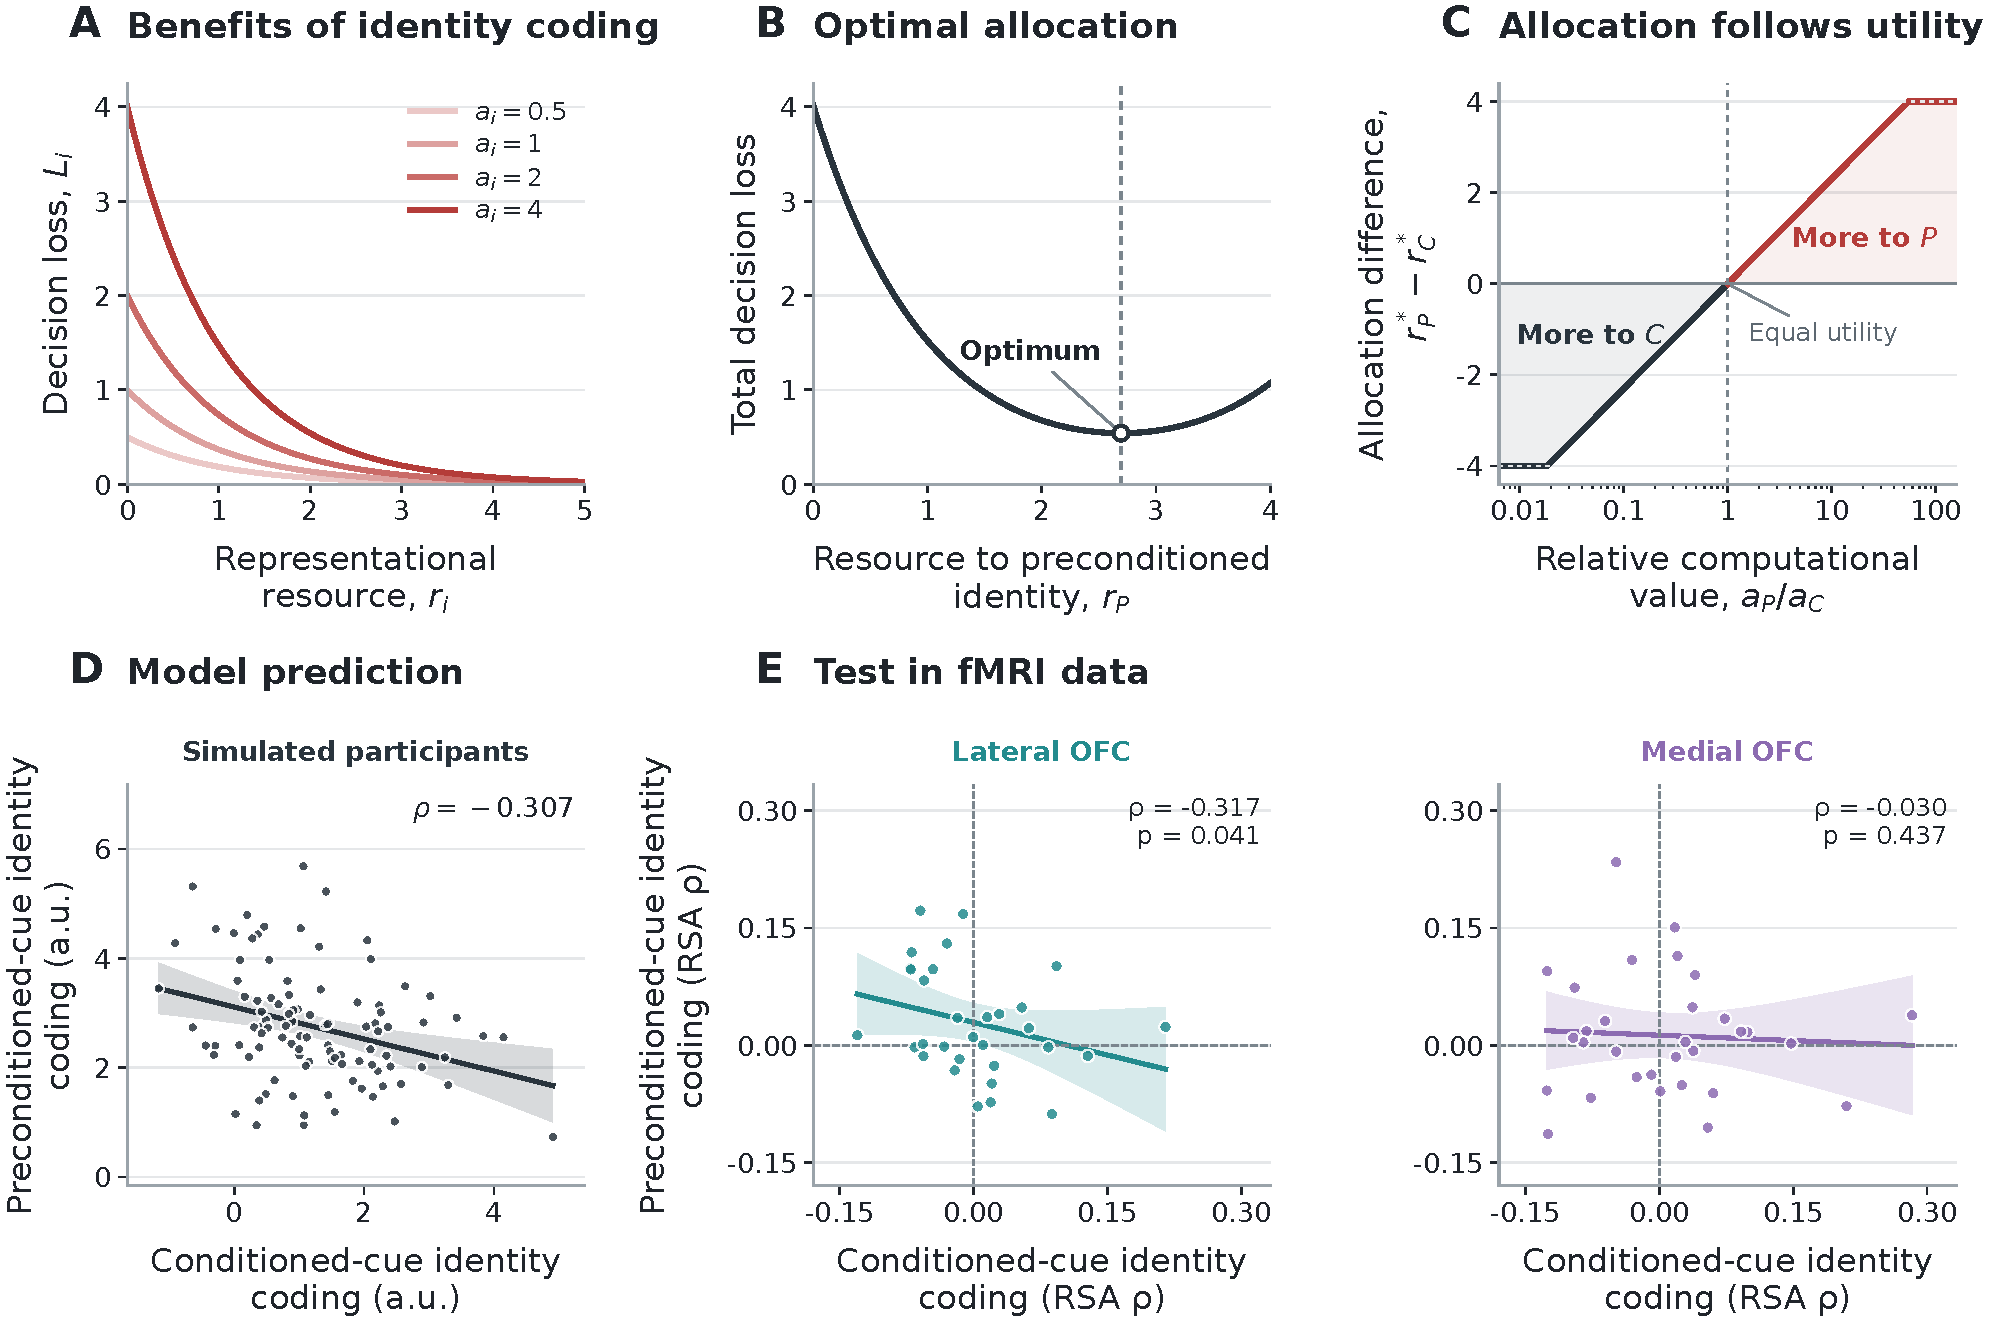
\includegraphics[width=0.95\linewidth]{../../fig/fig_model.pdf}
\caption{
\textbf{A resource-limited model of outcome-identity representation.}
\textbf{A. Benefits of identity representation.} Decision loss for cue $i$ decreases as representational resource $r_i$ is allocated to its outcome identity, according to $L_i=a_i e^{-r_i}$. Larger values of $a_i$ indicate a greater computational cost of weak identity representation, while the exponential form produces diminishing returns.
\textbf{B. Optimal allocation.} When inferred or preconditioned cues ($P$) and directly conditioned cues ($C$) share a finite representational budget, $r_P+r_C=R$, total decision loss is minimized by allocating resources according to their relative computational value. For the illustrative parameters $R=4$, $a_P=4$, and $a_C=1$, the optimum is $r_P^*=2.69$ and $r_C^*=1.31$.
\textbf{C. Allocation follows utility.} The optimal allocation difference is $r_P^*-r_C^*=\log(a_P/a_C)$ for interior solutions and is bounded by $\pm R$ because allocations must be nonnegative. Positive values indicate greater allocation to preconditioned cues ($P$), and negative values indicate greater allocation to conditioned cues ($C$). Thus, preferential representation of inferred outcomes emerges when their explicit identity representation has greater computational value ($a_P>a_C$); it is not imposed by cue category.
\textbf{D. Model prediction.} A shared budget predicts a negative relationship between direct and inferred identity representations across simulated participants. For 100 participants, $\log(a_P/a_C)$ was sampled from $\mathcal{N}(\log 4,1.2^2)$, and independent Gaussian measurement noise (standard deviation $0.75$) was added to each optimal allocation. Points show simulated representational strengths in arbitrary units, yielding Spearman $\rho=-0.307$. Parameters are illustrative and were not fitted to the fMRI results.
\textbf{E. Test in fMRI data.} Participant-level odor-identity RSA coefficients for conditioned and preconditioned cues were correlated across participants within lateral OFC (teal) and medial OFC (purple; $n=31$ for each region). The association was negative in lateral OFC (Spearman $\rho=-0.317$, $p=0.041$) and was not significant in medial OFC ($\rho=-0.030$, $p=0.437$); $p$ values are from one-sided tests of negative associations. Dashed lines indicate zero RSA coefficients. In D and E, solid lines show descriptive linear least-squares fits, and shading indicates pointwise 95\% confidence intervals for the fitted mean response.
}
\label{fig-identity-simu}
\end{figure*}




\section*{Discussion}



\subsection*{Information content of inferred outcomes}

Our behavioral findings show that model-based inference in sensory preconditioning extends beyond the retrieval of scalar reward value to include information about specific outcome identity. Selective satiation reduced choices not only for directly conditioned cues associated with the devalued odor, but also for preconditioned cues that had never been directly paired with that odor. Because the value of the visual cues themselves was never directly updated after satiation, this transfer of devaluation to preconditioned cues requires access to information about the specific outcome predicted through the learned associative chain. These findings extend previous evidence that responding to preconditioned cues is sensitive to outcome devaluation in rodents \cite{hart20} and complement human work showing that OFC activity during sensory preconditioning contains information about inferred outcomes \cite{wang2020interactions}. 


Our cross-task decoding results further suggest that inferred outcome expectations involve reactivation of outcome representations. A classifier trained to distinguish food odors during smelling successfully identified the expected odor from lateral OFC responses to preconditioned cues, even though no odors were delivered during the probe test. Previous studies showed that reward anticipation and receipt evoke similar neural representations of reward value in OFC \cite{RN1}, and that this similarity develops as cue--outcome associations are learned \cite{kahnt2011decoding}. Our findings extend this account to specific outcome identities inferred through separately learned associations. Because preconditioned cues had never been directly paired with the odors, these results suggest that associative inference can reinstate representations of outcomes that have not been directly experienced with the current cue.


\subsection*{Adaptive representation of reward identity in lateral OFC}

Our neural findings further suggest that reward-identity representations in lateral OFC are not expressed uniformly across all reward-predictive cues. Previous studies using directly learned cue--outcome associations have consistently identified identity-specific reward representations in lateral OFC, including representations that are updated by selective devaluation and predict subsequent goal-directed choices \cite{howard2015identity,howard2017identity,howard2018identity,liuyaoatt24,witkowski2026identity}. In the present task, however, identity information in lateral OFC was preferentially expressed for preconditioned cues, whose outcomes had to be inferred through associative structure, rather than for conditioned cues whose outcome identities had been directly learned. Thus, the present findings do not simply extend previous work by showing that lateral OFC represents another class of reward predictor. Instead, they suggest that the content of lateral OFC representations may depend on the computational demands imposed by the current task.

This interpretation is consistent with cognitive-map accounts proposing that OFC represents task-state information that is relevant but may not be directly observable for ongoing learning and decision making \cite{wilson2014orbitofrontal,schuck2016human,niv2019learning}. A central problem for such accounts is determining which of the many available features should be included in the task-state representation. Our resource-limited model provides one possible principle: detailed information about outcomes should be represented where doing so provides the greatest marginal computational benefit. Under a cost on representational resources, this difference can make explicit outcome-identity representations more valuable for preconditioned cues, producing the observed representational asymmetry without assuming that lateral OFC is intrinsically specialized for preconditioned cues.

More broadly, this account is compatible with prior work showing that working-memory constraints shape reinforcement learning, such that learning performance declines as the number of stimulus–response associations that must be maintained increases \cite{collins2012much,collins2018tortoise}. In our task, maintaining outcome information for both conditioned and preconditioned cues may impose a conceptually similar competition for limited representational resources.


\subsection*{Limitation and future directions}

One limitation is that the proposed resource-limited account is intended as a normative explanation of the observed representational asymmetry rather than as a model that was directly manipulated and tested in the present experiment. In particular, the behavioral cost of failing to recover the correct outcome identity, \(D_i\), was not experimentally varied and therefore remained effectively constant across conditions. Future studies could manipulate the consequences of errors, as well as the reliability of alternative routes for recovering outcome identity, to test whether representational resources shift in the manner predicted by the model. Such manipulations would provide a more direct test of whether lateral OFC representations are allocated according to the computational utility of explicit outcome information.


A second limitation is the modest sample size. Although the assignment of stimulus category—cartoon characters versus landmark places—to preconditioned and conditioned cues was fully counterbalanced across participants, the present sample may provide limited power to test whether stimulus category interacts with cue type or neural representation. Larger samples would allow these potential category-specific effects to be evaluated more directly. 

We did not find significant difference between the preconditioned cues and conditioned cue identity representation, so we could not make the conclusion saying that the lateral OFC regions did not represent conditioned cues at all and only represented preconditioned cues. 


\subsection*{Conclusions}

Together, our findings show that model-based inference in sensory preconditioning extends beyond scalar reward value to include the identity of specific expected outcomes. Selective devaluation altered choices for both directly conditioned and preconditioned cues, demonstrating that behavior toward indirectly related cues depends on access to specific outcome information. At the neural level, lateral OFC represented expected odor identity for preconditioned cues, whereas neither RSA nor cross-task decoding detected significant odor-identity representations for conditioned cues. vmPFC reflected the relative subjective values of expected outcomes. Our resource-limited model provides a possible framework for understanding how the computational benefit of outcome information could guide the allocation of representational resources. More broadly, these findings support a view of OFC as an adaptive cognitive map whose representational content is shaped by the information most useful for current behavior.




\matmethods{

\subsection*{Study participants}

Thirty-five healthy, right-handed participants with no history of major psychiatric or neuro-logical disorders provided written informed consent to participate in the study. One participant withdrew due to scheduling constraints, leaving 34 individuals who completed all experimental sessions. All participants fasted for approximately 2–4 hours before each study visit. Two participants were excluded from data analysis because they did not demonstrate learning during the conditioning task, rendering their data unsuitable for further analyses. One additional participant was excluded because of a persistent preference for clean-air cues and absent odor devaluation, suggesting limited engagement with the odor outcomes central to the study. The final sample comprised 31 participants (11 males, 20 females; ages 21–42, $M = 28.58$, $SD = 6.03$). The study protocol was approved by the NIDA-IRP Institutional Review Board (Study~\#001156) and registered on ClinicalTrials.gov (NCT05707806).



\subsection*{Study design}


This study used a modified sensory preconditioning paradigm combined with outcome devaluation. Participants first completed a preconditioning phase, during which they learned associations between pairs of visual cues (A1-B1, A2-B2, and C-D). For a given participant, cues A1, A2 and C were images of places whereas B1, B2 and D cues were cartoon characters (counterbalanced across participants). There were two sets of cue pairs, and each set comprised two A-B pairs (A1-B1 and A2-B2) and one C-D pair (Table~\ref{tab:cue-mapping}). This was followed by a conditioning phase, where participants learned associations between the second cue in each pair and a sweet (B1) or savory (B2) food odor, or no odor (D). Finally, participants completed a probe task in which they made choices among both conditioned and preconditioned cues, reflecting their preferences for the associated odors. The probe task was administered twice: once before and once after participants consumed a meal that was matched to either the sweet or the savory food odor (counterbalanced across participants).



\begin{table}[t]
\centering
\caption{Cue–outcome mapping structure for preconditioned cues, conditioned cues, and their associated odor outcomes. 
In this illustration, the sweet odor is paired with A1 and B1 for consistency with \autoref{fig-design}; 
in the actual experiment, the sweet–savory assignment was counterbalanced across participants.
}
\label{tab:cue-mapping}
\begin{tabular}{ccccc}
\hline
\textbf{Cue set} & \textbf{Preconditioned cue} & \textbf{Conditioned cue} & \textbf{Outcome} \\
\hline
Set 1 & $A1_{1}$ & $B1_{1}$ & sweet odor \\
Set 1 & $A2_{1}$ & $B2_{1}$ & savory odor \\
Set 1 & $C_{1}$ & $D_{1}$ & clean air \\
Set 2 & $A1_{2}$ & $B1_{2}$ & sweet odor \\
Set 2 & $A2_{2}$ & $B2_{2}$ & savory odor \\
Set 2 & $C_{2}$ & $D_{2}$ & clean air \\
\hline
\end{tabular}
\end{table}




\subsection*{Study sessions}

The study spanned three days, consisting of a stimulus selection session, Day 1, and Day 2. During the stimulus selection session, participants rated the images and odors. Day 1 included an MRI localizer scan followed by preconditioning training. Day 2 began with a brief preconditioning refresher (outside the scanner), followed by the conditioning task (three runs, inside the scanner) and two probe tasks (three runs each, inside the scanner), separated by the meal. Immediately before and after the meal, participants rated odor pleasantness and self-reported satiation. Day 2 concluded with a recognition memory task outside the scanner, followed by a post-task interview (see Supplementary Methods). The interval between the stimulus selection session and Day~1 was, on average, \(8.03 \pm 11.13\) days, and the interval between Day~1 and Day~2 was \(7.41 \pm 5.06\) days.


\subsubsection*{Stimulus selection session}

In the stimulus selection session, participants first completed an image rating task outside the scanner, in which they evaluated a series of character images followed by place images, indicating how much they liked each one. The purpose of this task was to identify images with neutral---or as similar as possible---liking ratings so that these images could be used as visual cues, ensuring that subsequent preference-based choices would primarily reflect participants' odor preferences rather than any preexisting preferences for particular visual stimuli. Participants rated each image three times, and we selected eight character images and eight place images based on their average ratings.


Next, participants completed an odor rating and selection procedure in which they evaluated the pleasantness and intensity of ten food odors. On each trial, participants smelled one odor for 2 s and then rated how much they liked it using a visual analog scale ranging from “Most Disliked Sensation Imaginable” to “Most Liked Sensation Imaginable.” Ratings were made by positioning a cursor along the scale. Each odor was presented three times in a pseudo-randomized order, and the three ratings for each odor were averaged. Based on these averaged ratings, two odors—one savory and one sweet—were selected for each participant. We selected odors that were rated above neutral and as closely matched in pleasantness as possible, and at least medium in perceived intensity. These individualized odors served as the reward outcomes for the remainder of the experiment.


\subsubsection*{Study day 1 – Localizer (fMRI)}

On study day 1, participants completed a series of fMRI localizer scans designed to obtain neural responses to all visual and olfactory stimuli before any associative learning occurred. The session included two odor localizer runs, four character localizer runs, and four place localizer runs. 


\paragraph*{Odor localizer}

Participants completed two runs of the odor localizer, in which each trial consisted of a 2\,s sniff cue followed by 2\,s of odor delivery (one of the two participant-specific food odors or clean air), separated by a jittered 9--13\,s ITI. Each run contained 30 trials (3 odor types $\times$ 10 repetitions). Participants were instructed to inhale deeply at the sniff cue while minimizing head and body movement.






\subsubsection*{Study day 1 – Preconditioning training}

On Day 1, following the localizer MRI scans, participants completed preconditioning training outside the scanner. During this phase, they learned six deterministic associations comprising six cue pairs: two A1–B1 pairs, two A2–B2 pairs, and two C–D pairs. For each participant, the A1, A2, and C cues were places, whereas the B1, B2, and D cues were characters. Participants were instructed to learn and remember which place was associated with each character. Instead of a passive viewing paradigm, we implemented a choice-based design to facilitate active engagement and promote more robust encoding of the paired associations \cite{bunsey1996conservation}. 


Each trial began with a 3\,s presentation of the first cue (e.g., A1), followed by a 0.3\,s gap and then a 3\,s presentation of two possible second cues, one of which was the correct associate (e.g., B1), whereas the incorrect cue was from one of the other cue pairs within the same cue set (i.e., B2 or D). During this 3\,s choice period, participants indicated which of the two cues was associated with the preceding cue A1 by pressing left or right arrow key. Trials were separated by a jittered 3–8\,s inter-trial interval. Feedback (correct, incorrect) was provided after each choice. Whether the character or the place served as cue A1 and B1 (appeared first and second) was counterbalanced across participants as part of the experimental design.


Each run comprised 24 trials (6 cue pairs $\times$ 2 incorrect alternatives drawn from the same cue set $\times$ left/right balancing). Participants completed 3--5 runs in total, with the task terminating early if they achieved $\geq 90\%$ accuracy after the third or fourth run.


\subsubsection*{Study day 2 – Main task}



\paragraph*{Preconditioning refresher}

Day 2 began with a brief preconditioning refresher outside the scanner to reinforce the character–place associations learned on Day 1. Participants were allowed up to three refresher runs; those who achieved greater than 90\% accuracy after the first or second run skipped the remaining runs. The structure of each run was identical to the preconditioning training on day 1. Of the 32 participants retained for analysis, 30 met the accuracy threshold after one run, whereas only 2 participants required a second run.


\paragraph*{Conditioning task}

In the conditioning task, participants viewed the second cue of each pair (i.e., B1, B2, and D) and predicted which odor (or clean air) would follow. Cues B1 and B2 were associated with the sweet and savory odor, respectively, whereas cues D were associated with no odor. To encourage retrieval of the associated, absent preconditioned cues (A1, A2 and C), participants were provided with a cover story instructing them to think about the related cue while making their predictions. Each trial began with a 2\,s presentation of a conditioned cue, followed by a 3\,s prediction period during which the cue remained on the screen and three odor abbreviations were displayed. Participants indicated which odor they expected. After a 4\,s delay following the prediction period, the associated odor (or clean air) was delivered for 2\,s. If no response was made, no odor was delivered and a “too slow” message appeared. Trials concluded with a jittered 4--10\,s inter-trial interval. Each run comprised 36 trials (6 cues $\times$ 6 orderings of odor names).


\paragraph*{Probe task (pre-meal and post-meal)}

In the probe task, administered both before and after the meal, participants made choices between two sequentially presented cues based on which associated odor (or clean air) they preferred to smell. The two sequentially presented cues could either be two conditioned cues (i.e., B1 vs. B2, B1 vs. D, or B2 vs. D) or two preconditioned cues (i.e., A1 vs. A2, A1 vs. C, or A2 vs. C). Participants were informed that no odors would be delivered during the task; instead, five trials would be randomly selected and the odor corresponding to their choice would be delivered at the end of the experiment.


Each trial began with a 3\,s presentation of the first cue (cue\,1), followed by a jittered 4--10\,s interval before the second cue (cue\,2) appeared for 3\,s. Participants then had 2\,s to indicate their choice, after which the trial ended with a jittered 4--10\,s inter-trial interval. Each run comprised 24 trials (6 pairwise choice pairs $\times$ 2 cue sets $\times$ left/right balancing).




\paragraph*{Meal consumption}

Between the pre- and post-meal probe tasks, participants exited the scanner and consumed a meal matched to one of the two food odors (sweet or savory, counterbalanced across participants). Participants were given 15\,minutes and instructed to eat until they felt very full. Additional meal details and caloric intake are reported in Supplementary Methods.


\paragraph*{Odor pleasantness ratings}

Participants rated the pleasantness of each odor before and after the meal using a horizontal slider ranging from –4 (very unpleasant) to +4 (very pleasant) in 0.5-point increments. Each odor was rated three times, and the average of the three ratings was used in subsequent analyses. Because of an operational error, pleasantness, hunger, and satiety ratings were unavailable for one participant, leaving 30 participants for these analyses.




\subsection*{Task stimuli}

\paragraph*{Visual stimuli}

We used two categories of visual stimuli—cartoon characters and landmark places—along with ten food-related odors. The visual stimulus set comprised 30 familiar cartoon characters (e.g., Jerry Mouse, Snoopy, Charmander) and 30 commonly recognizable places (e.g., office buildings, university campuses, bridges). Images were selected to avoid strong positive or negative affective content and to minimize any real-world associations with specific odors. For cartoon characters, we also excluded images with pronounced lateral gaze directions to prevent potential biases in participants’ left–right choices during the task. All images were converted to grayscale to reduce visual saliency and to ensure that any differences in preference or neural representation were not driven by low-level perceptual features.

\paragraph*{Odor stimuli and delivery}

We used five savory odors (potato chip, garlic, cheddar, pizza, tuna) and five sweet odors (strawberry, chocolate, apple cinnamon, peach, vanilla). Food odors were sourced from several commercial suppliers: Takasago International Corporation (Tokyo, Japan), International Flavors \& Fragrances (New York, NY), The Flaming Candle (Strongsville, OH), The Candlemaker’s Store (Butler County, OH), and the Midwest Sea Salt Company (West Chester, OH).


We used a custom-built computer-controlled olfactometer to deliver food odors with precise timing directly to nasal masks worn by subjects. This olfactometer directed medical-grade air through the headspace of amber bottles containing liquid solutions of food odors, maintaining a constant flow rate of 3.2~L/min. Using two independent mass flow controllers (Alicat, Tucson, AZ), the olfactometer enabled the dilution of odorized air with odorless air. Throughout the experiment, a constant stream of odorless air was delivered to subjects’ noses. Odorized air was mixed into this airstream at specific time points, while ensuring no impact on the overall flow rate and preventing any alteration in somatosensory stimulation.


\subsection*{MRI data acquisition}


MRI data were acquired on a Siemens 3T Prisma-Fit system using a 32-channel head coil. Functional images were collected with a multi-echo gradient-echo EPI sequence (TR = 1.5\,s; TE$_1$--TE$_4$ = 12.60, 29.16, 45.72, and 62.28\,ms; flip angle = 67$^\circ$; in-plane voxel size = 2.51~$\times$~2.51\,mm; slice thickness = 2.5\,mm (no gap); matrix size = 86~$\times$~86 voxels; field of view = 216~$\times$~216\,mm; 60 axial slices acquired in an interleaved order; multiband acceleration factor = 4). The short first echo time helps reduce susceptibility-induced signal dropout in orbitofrontal cortex, as demonstrated in previous resting-state and task-based fMRI studies \cite{RN619,RN524,kirlutpos16,zhao24img}. High-resolution T1-weighted structural images (1\,mm isotropic) were acquired on Day~1 to facilitate spatial normalization.

Across the two study days, functional MRI runs varied in length depending on the task. On Day~1, the odor localizer scan comprised 320 volumes, and each character and place localizer run comprised 244 volumes. On Day~2, the odor prediction task consisted of 404 volumes, and each pre- and post-meal probe run contained 372 volumes.


\subsection*{Multi-echo MRI data processing}


Preprocessing of the multi-echo fMRI data followed the procedures described in our recent work \cite{liu2025distinct}. First, all functional images from the shortest echo across all fMRI runs were realigned to the first volume of the first echo using SPM12, and the resulting voxel-to-world mapping matrix was applied to the other three echoes, volume by volume. All functional images were then resliced for each echo. Next, the images across the four echoes were combined using temporal signal-to-noise ratio (tSNR) weighting, following parallel-acquired inhomogeneity desensitized (PAID) approach \cite{RN524}. Specifically, voxel-wise tSNR maps were computed for each echo, multiplied by the echo time (TE), and normalized across the four echoes to generate weight maps. These weight maps were then used to combine the resliced images by multiplying each volume by its respective weight map. Finally, the combined multi-echo data were coregistered, normalized to MNI space, resampled to 2 mm isotropic resolution, and smoothed with a 2\,mm full-width at half-maximum (FWHM) Gaussian kernel, all using SPM12.



\subsection*{Sniff recording and analysis}

We measured subjects’ nasal airflow (i.e., sniffing) directly at the nose using a nasal mask connected to a respiratory flow head and spirometer. Nasal airflow was recorded with PowerLab equipment (ADInstruments, Dunedin, New Zealand) at a sampling rate of 1\,kHz. Airflow traces for each fMRI run were preprocessed by smoothing with a 250\,ms moving window, down-sampling to 10\,Hz, applying a high-pass filter (50\,s cutoff) to remove slow drifts, normalizing each run by subtracting the mean and dividing by the standard deviation, and finally down-sampling to match the fMRI repetition time of 1.5\,s (TR). Sniff volume was computed as the integral of the nasal airflow. Nasal airflow, sniff volume, and their squared terms were included as nuisance regressors in the fMRI GLM analyses. Additional nuisance regressors accounting for head motion and image artifacts are described in Supplementary Methods.


\subsection*{Behavioral data analysis}

We analyzed behavioral performance from the preconditioning task, the conditioning task, as well as the pre- and post-meal probe tasks. We excluded data from two participants whose run-wise accuracies in the conditioning task were consistently below 0.40. Among the remaining 32 participants, accuracy in the final run of conditioning was high: all participants achieved at least 0.75, with a mean of 0.94 and a standard deviation of 0.068. These results indicate robust learning of the cue–odor (or clean-air) associations by the end of the conditioning task. Details of behavioral measure calculation, trial inclusion, and statistical testing are provided in Supplementary Methods.



\subsection*{Single-presentation GLMs}


We estimated single-presentation GLMs for the premeal and postmeal probe tasks using the least-squares-separate approach \cite{mumford2012deconvolving}. A separate GLM was fitted for each cue presentation, modeling the target cue at its onset with a duration of 3 s and pooling all other cue presentations within the same run into a second regressor. Both cue positions were estimated, yielding two GLMs per trial. Each model additionally included decision periods, modeled with a duration of 2 s; separate left- and right-hand button-press regressors, modeled as zero-duration events; and the nuisance regressors described above. Models were estimated on resliced, coregistered, normalized functional EPIs smoothed with a 2 mm FWHM Gaussian kernel. A high-pass filter with a cutoff of 128 s was applied.

Single-trial beta estimates were also obtained from the passive odor localizer using the least-squares-separate approach. A separate GLM was fitted for each presentation, with the target presentation modeled as a zero-duration event at sniff-cue onset and all remaining presentations within the same run pooled into a second regressor. Models used the same preprocessed functional images and nuisance regressors described above, with a high-pass filter cutoff of 128 s. Beta estimates for the two food odors were used to train the cross-task decoder.



\subsection*{Representation similarity analysis}
\label{rsa-probe}

We conducted a region-of-interest (ROI) RSA examining odor-associated representational structure in the premeal probe task, before devaluation could introduce confounding changes in odor value. Analyses used the two bilateral orbitofrontal cortex (OFC) regions defined below.

Single-image beta estimates were selected for the first cue presentation of each trial. Conditioned and preconditioned cues were analyzed separately, each comprising four odor-predictive cue identities across the two stimulus sets. Clean-air-associated cues were excluded. Individual presentation patterns were retained without averaging across trials or runs. Each cue subset ordinarily contained 24 samples across three runs, with two presentations of each cue per run. Participant 36 contributed 16 samples from two runs.

Within each ROI and cue subset, voxels with nonfinite values in any selected sample were removed. Each voxel’s responses were mean-centered across the selected samples within each run. Neural representational dissimilarity matrices were constructed using one minus the Pearson correlation between activity patterns. An odor-identity model assigned zero to pairs associated with the same odor and one to pairs associated with different odors. Correspondence between neural and model dissimilarities was assessed using Spearman correlation, retaining only pairs of samples acquired in different runs. Group inference used one-sided one-sample t tests of participant-level Spearman coefficients against zero. 

Within each OFC ROI, participant-level odor-identity RSA coefficients for conditioned and preconditioned cues were correlated across participants using Spearman rank correlation. Negative associations were assessed using one-sided tests, with an uncorrected significance threshold of $p < 0.05$.


\subsection*{Cross-task decoding of odor identity}

We tested whether multivoxel representations of perceived odor identity generalized to odor-associated visual cues. Analyses used the same two bilateral OFC regions as RSA. For each participant and ROI, a linear support vector machine with a fixed regularization parameter of C = 1 was trained to distinguish the two odors using single-trial beta patterns from the passive odor task conducted before associative learning. Training included 40 odor presentations across two runs, with 20 presentations per odor. Clean-air trials were excluded.

The classifier was subsequently tested on single-image beta patterns from the premeal probe task, during which no odors were delivered. Only the first cue presentation of each trial was included. Conditioned and preconditioned cues were evaluated separately, retaining four odor-predictive cue identities per subset across the two stimulus sets. Each subset ordinarily contained 24 samples across three runs; participant 36 contributed 16 samples from two runs. Test labels indicated the odor associated with each cue.

For each participant, ROI, and cue subset, voxels with nonfinite values in any training or test sample were excluded. Voxel responses were z-scored across samples separately within each run and task, with the two stimulus sets pooled within each probe run. Normalization statistics were calculated independently for the passive odor and probe datasets. The classifier was fitted using both passive odor runs and applied to the probe patterns without further fitting or hyperparameter selection. Decoding accuracy was calculated as the mean proportion of correct classifications across the two odor identities. One-sided one-sample t tests assessed whether participant-level decoding accuracy exceeded the chance level of 50\%.

\subsection*{Region-of-interest definition}

Analyses used two independently defined bilateral orbitofrontal cortex (OFC) regions from the connectivity-based K = 2 parcellation: medial/posterior-lateral OFC (hereafter medial OFC) and central/anterior-lateral OFC (hereafter lateral OFC) \cite{kahnt2012connectivity}. The parcellation map was resampled to the 2 mm isotropic analysis grid using nearest-neighbor interpolation. Each region was then intersected with a gray-matter mask derived from the SPM12 gray-matter tissue probability map thresholded at probability $>0.1$. The same ROI definitions were used for odor-identity RSA and cross-task decoding.




}



\showmatmethods{} % Display the Materials and Methods section

\dataavail{Anonymized behavioral data and analysis and simulation code are available at https://github.com/QingfangLiu/project-spcd. Additional data are available from the corresponding author upon reasonable request, subject to applicable institutional and participant-consent restrictions.}


\acknow{This work was supported by National Institute on Deafness and Other Communication Disorders grant R01DC015426 (to T.K.) and the Intramural Research Program at the National Institute on Drug Abuse (ZIA DA000642 to T.K. and DA000587 to G.S.), as well as by a fellowship from the National Institutes of Health (NIH) Center on Compulsive Behaviors (to Q.L.). This research was also supported in part by the Intramural Research Program of the National Institutes of Health (NIH). The contributions of the NIH authors are considered “works of the United States government.” The findings and conclusions presented in this paper are those of the authors and do not necessarily reflect the views of the NIH or the US Department of Health and Human Services.}


\showacknow{} % Display the acknowledgments section




\bibsplit[17]
%Use \bibsplit to split the references from the body of the text. Value "[3]" represents the number of reference in the left column (Note: Please avoid single column figures & tables on this page.)

% Bibliography
\bibliography{sn-bibliography}

\end{document}
